% Four Major Mathematics Awards — Cross-Reference (Beamer)
% Fields · Wolf · Abel · Chern，交叉获奖名录
% 版式参照 fields_beamer/fields_medal_laureates_beamer.tex
% Compile with: xelatex math_awards_allinone_beamer.tex

\documentclass[aspectratio=169,9pt]{beamer}

% ---- Theme ----
\usetheme{default}
\usecolortheme{default}
\setbeamertemplate{navigation symbols}{}
\setbeamertemplate{footline}{%
  \hfill{\tiny\color{mutedgray}\insertframenumber/\inserttotalframenumber}\hspace*{6pt}\vspace{4pt}%
}
\setbeamertemplate{frametitle}{%
  \vspace{4pt}%
  \noindent\hspace*{8pt}{\large\bfseries\color{headerblue}\insertframetitle}%
  \hfill
  \raisebox{-1pt}{\footnotesize\color{mutedgray} 四大奖交叉名录 · Fields · Wolf · Abel · Chern}%
  \hspace{8pt}%
  \vspace{2pt}%
  \par\noindent\hspace*{8pt}\textcolor{headerbg}{\rule{0.95\textwidth}{0.6pt}}%
  \vspace{-2pt}%
}

% ---- Fonts & Language ----
\usepackage{fontspec}
\usepackage{xeCJK}
\setCJKmainfont{PingFang SC}[BoldFont=PingFang SC Semibold]
\setCJKsansfont{PingFang SC}
\setmainfont{Helvetica Neue}[BoldFont=Helvetica Neue Bold]
\setsansfont{Helvetica Neue}

% ---- Packages ----
\usepackage{booktabs}
\usepackage{array}
\usepackage{tikz}
\usepackage{amssymb}
\usepackage{colortbl}
\usepackage{graphicx}

% ---- Colors ----
\definecolor{headerblue}{RGB}{41,65,122}
\definecolor{headerbg}{RGB}{200,215,240}
\definecolor{yearcolor}{RGB}{180,50,50}
\definecolor{fieldcolor}{RGB}{30,100,60}
\definecolor{mutedgray}{RGB}{100,100,100}
\definecolor{slidebg}{RGB}{253,254,255}
% ---- Per-award brand colors (match math_awards_allinone) ----
\definecolor{fieldsclr}{RGB}{41,65,122}   % Fields — 深蓝
\definecolor{wolfclr}{RGB}{180,120,0}     % Wolf   — 金棕
\definecolor{abelclr}{RGB}{150,40,90}     % Abel   — 紫红
\definecolor{chernclr}{RGB}{15,110,92}    % Chern  — 翡翠绿
\definecolor{triplebg}{RGB}{255,224,224}  % 三奖高亮
\definecolor{doublebg}{RGB}{223,233,250}  % 双奖高亮

% ---- Beamer Colors ----
\setbeamercolor{background canvas}{bg=slidebg}
\setbeamercolor{title}{fg=headerblue}

% ---- Custom Commands ----
% 奖项徽标：追加在姓名后
\newcommand{\Fbadge}{\textsuperscript{\normalfont\tiny\color{fieldsclr}$\blacklozenge$\kern-0.5pt F}}
\newcommand{\Wbadge}{\textsuperscript{\normalfont\tiny\color{wolfclr}$\bigstar$\kern-0.5pt W}}
\newcommand{\Abadge}{\textsuperscript{\normalfont\tiny\color{abelclr}$\blacktriangle$\kern-0.5pt A}}
\newcommand{\Cbadge}{\textsuperscript{\normalfont\tiny\color{chernclr}$\blacksquare$\kern-0.5pt C}}

% Cross-award row: #1=英文名 #2=中文名 #3=徽标串 #4=各奖年份 #5=国籍 #6=领域
\newcommand{\crow}[6]{%
  {\bfseries\color{headerblue}#1}#3\newline{\scriptsize\color{mutedgray}#2}
  & {\scriptsize\color{yearcolor}#4} & {\scriptsize #5} & {\scriptsize\color{fieldcolor}#6} \\[2.5pt]
}

% Category header row inside table
\newcommand{\catrow}[2]{%
  \rowcolor{#2}
  \multicolumn{4}{l}{\raisebox{0pt}[1.1em][0.3em]{\bfseries\color{headerblue}\small #1}} \\[0.5pt]
}

% ---- Document ----
\begin{document}

% ============================================================
% Title Slide
% ============================================================
\begin{frame}
\vfill
\begin{center}
  {\Huge\bfseries\color{headerblue} 数学「大满贯」俱乐部 · 四大奖项交叉名录}\\[8pt]
  {\Large\color{headerblue} Fields · Wolf · Abel · Chern}\\[6pt]
  {\normalsize\color{mutedgray} 双料冠军 · 三冠传奇 · 全满贯得主 · 共 33 人}\\[12pt]
  {\small\color{mutedgray} 1936–2026 · 交叉获奖标注 · 附中文名字}\\[10pt]
  {\footnotesize 徽标：%
    {\color{fieldsclr}$\blacklozenge$F} 菲尔兹奖\quad
    {\color{wolfclr}$\bigstar$W} 沃尔夫奖\quad
    {\color{abelclr}$\blacktriangle$A} 阿贝尔奖\quad
    {\color{chernclr}$\blacksquare$C} 陈省身奖章}
\end{center}
\vspace{6pt}
\begin{center}
  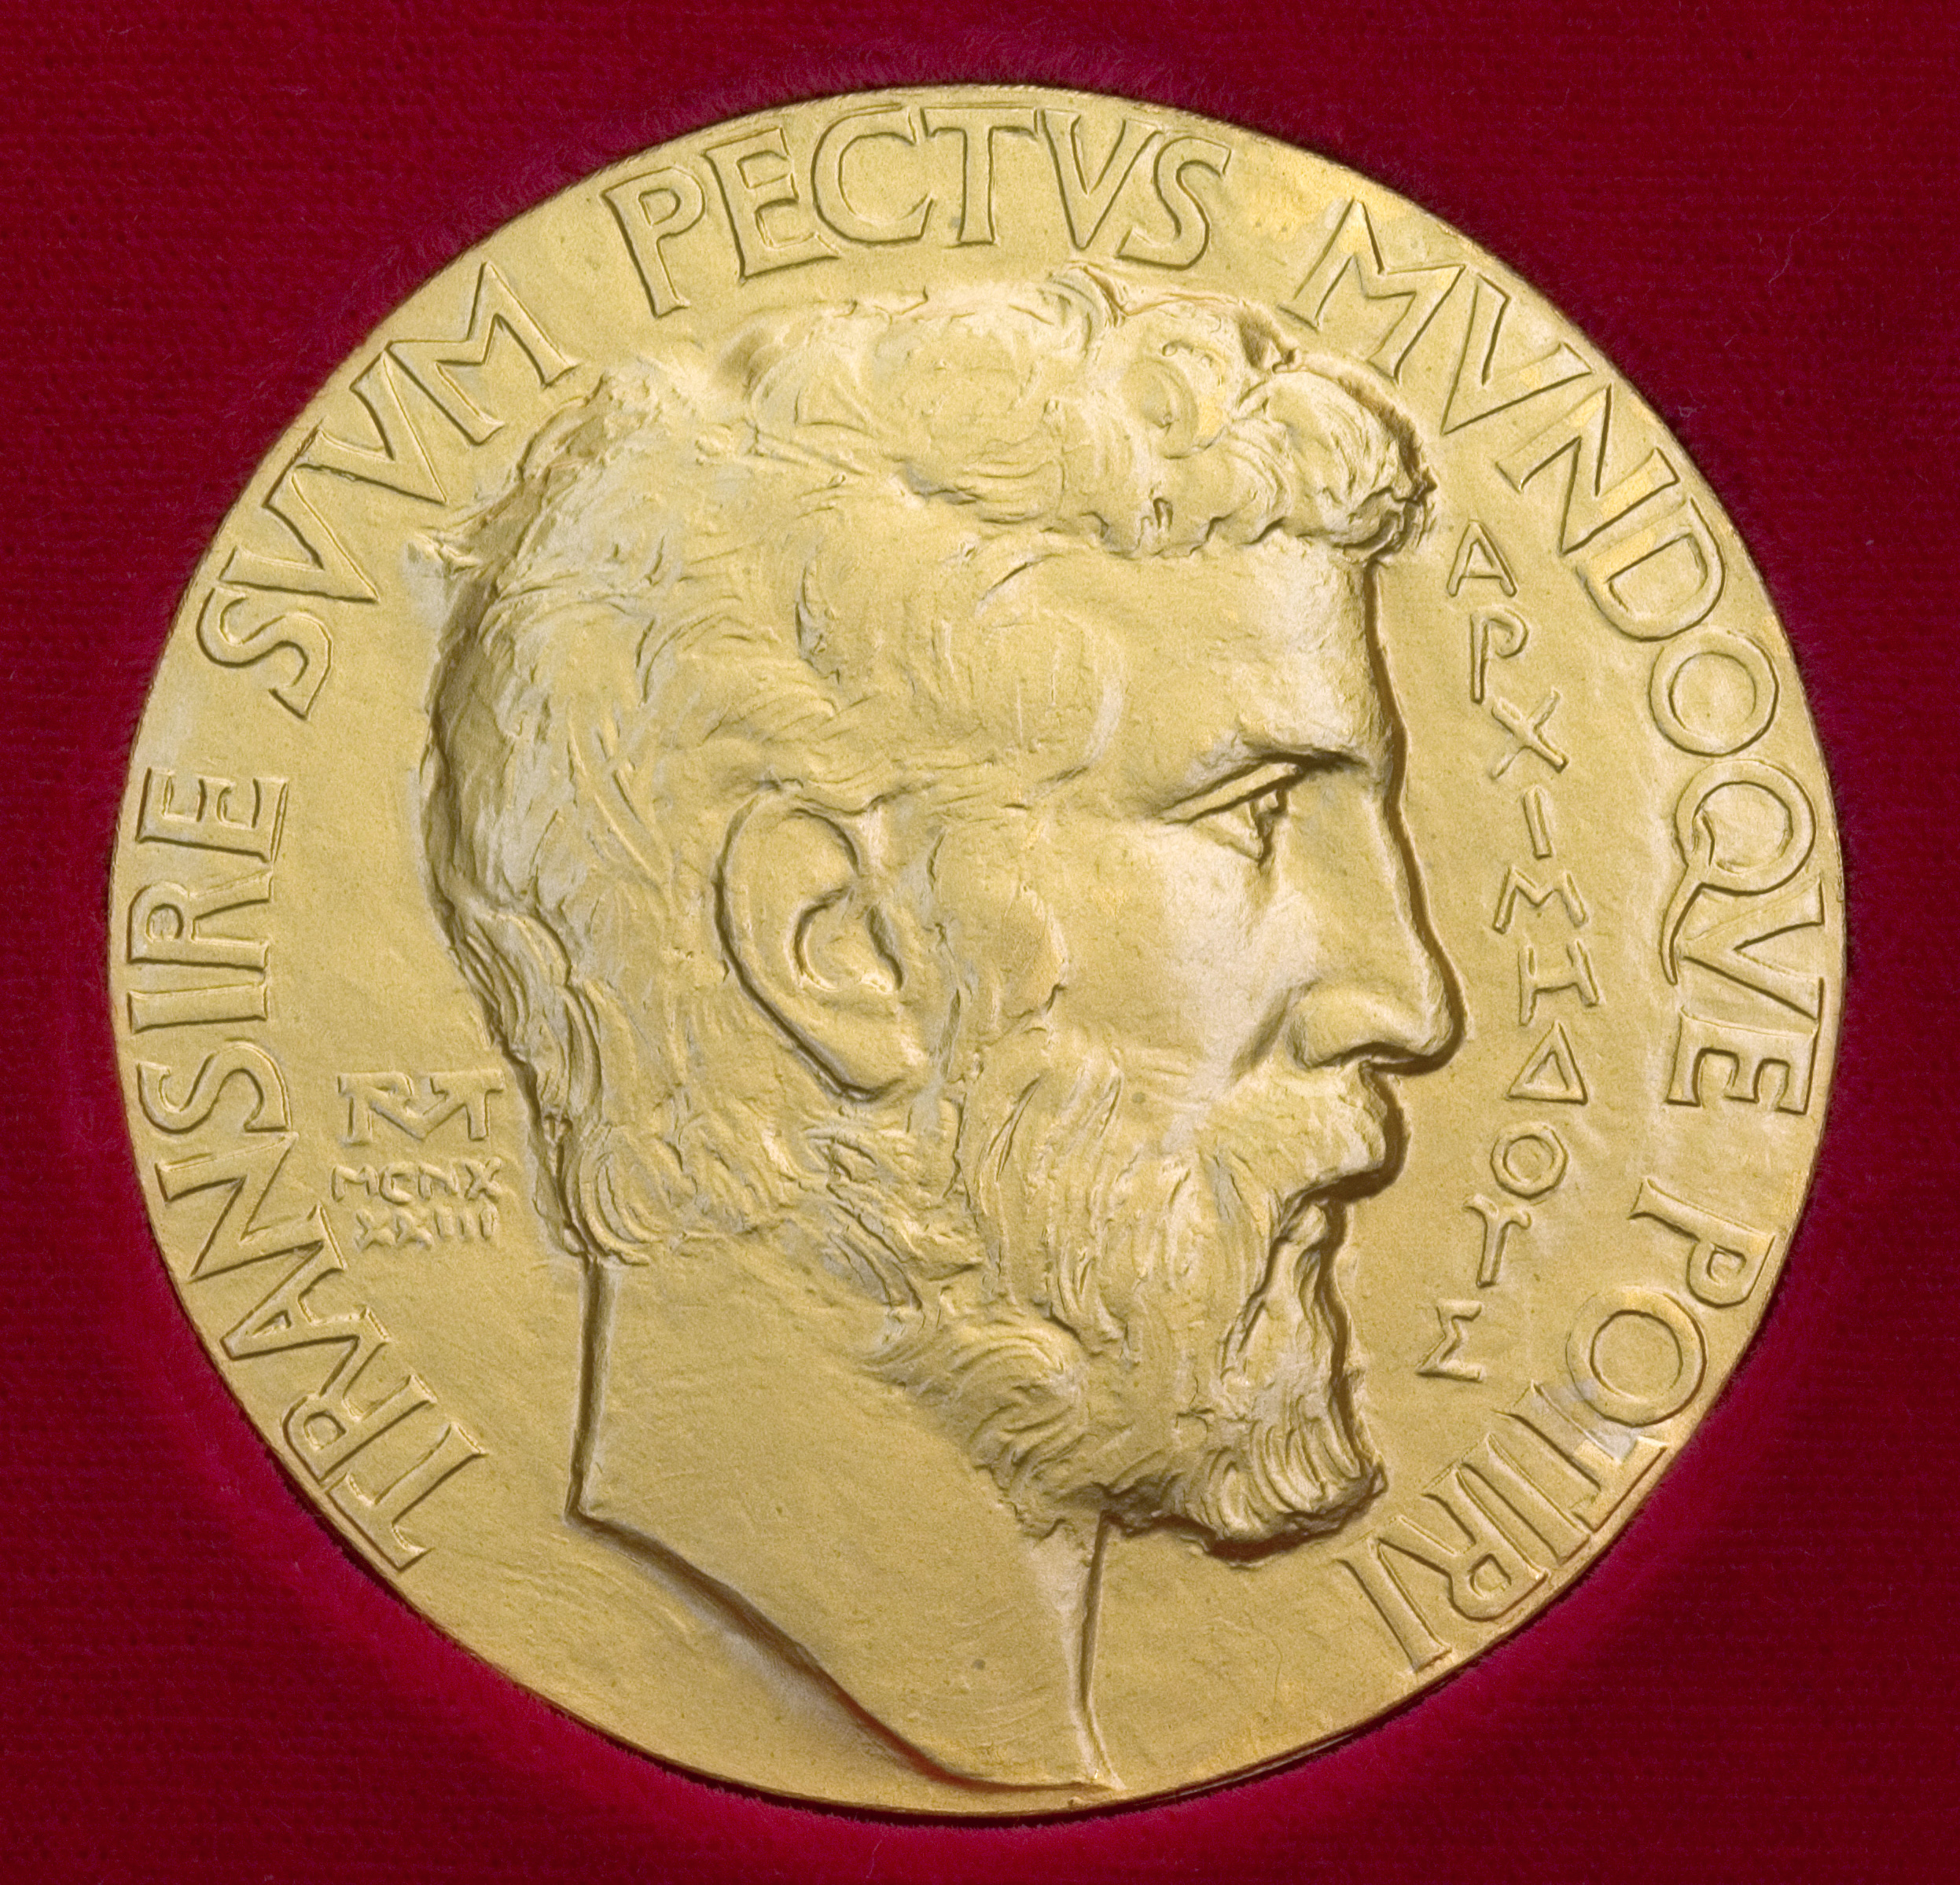
\includegraphics[height=3cm]{cover/FieldsMedalFront_hires.jpg}\hspace{2cm}
  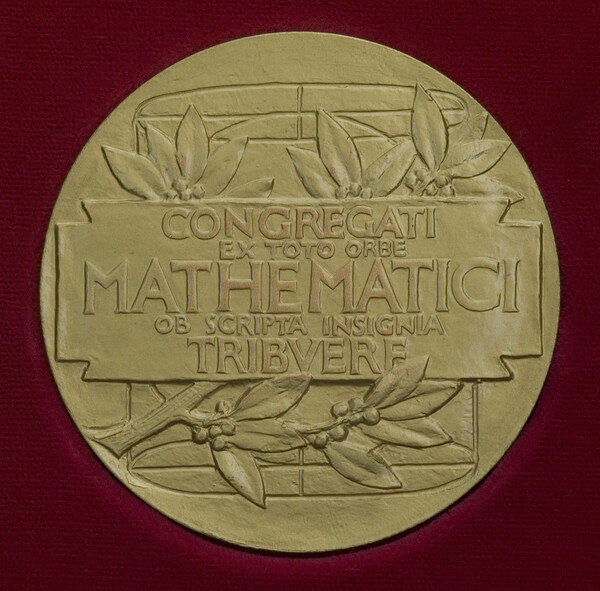
\includegraphics[height=3cm]{cover/FieldsMedalBack_600px.jpg}
\end{center}
\vspace{10pt}
\begin{center}
  {\small\color{mutedgray}\itshape 名字后徽标越多，代表其横跨的顶级奖项越多；下列按获奖组合分类。}
\end{center}
\vfill
\end{frame}

\begin{frame}{★★★ 三奖得主 · Fields + Wolf + Abel}
\vspace{-2pt}
\centering
\scriptsize
\begin{tabular}{@{}
  >{\raggedright}m{3.6cm}
  >{\raggedright}m{2.9cm}
  >{\raggedright}m{1.5cm}
  >{\raggedright\arraybackslash}m{4.3cm}
@{}}
\toprule
\rowcolor{headerbg}
\textbf{姓名（徽标）} & \textbf{获奖年份} & \textbf{国籍} & \textbf{研究领域} \\
\midrule
\catrow{★★★ 三奖得主 · Fields + Wolf + Abel}{triplebg}
\crow{Jean-Pierre Serre}{让-皮埃尔·塞尔}{\Fbadge\Wbadge\Abadge}{F 1954 · W 2000 · A 2003}{法国}{代数拓扑、代数几何、数论；史上最年轻菲尔兹奖（27 岁），首届阿贝尔奖}
\crow{John Milnor}{约翰·米尔诺}{\Fbadge\Wbadge\Abadge}{F 1962 · W 1989 · A 2011}{美国}{微分拓扑、异国球面、K 理论、动力系统}
\crow{John G. Thompson}{约翰·汤普森}{\Fbadge\Wbadge\Abadge}{F 1970 · W 1992 · A 2008}{美国}{有限群论、奇阶定理、有限单群分类}
\crow{Pierre Deligne}{皮埃尔·德利涅}{\Fbadge\Wbadge\Abadge}{F 1978 · W 2008 · A 2013}{比利时}{代数几何、Weil 猜想、Hodge 理论}
\crow{Grigory Margulis}{格里戈里·马尔古利斯}{\Fbadge\Wbadge\Abadge}{F 1978 · W 2005 · A 2020}{苏联/美国}{Lie 群格、刚性理论、遍历理论}
\bottomrule
\end{tabular}
\end{frame}

\begin{frame}{★★ 双奖 · Fields + Wolf}
\vspace{-2pt}
\centering
\scriptsize
\begin{tabular}{@{}
  >{\raggedright}m{3.6cm}
  >{\raggedright}m{2.9cm}
  >{\raggedright}m{1.5cm}
  >{\raggedright\arraybackslash}m{4.3cm}
@{}}
\toprule
\rowcolor{headerbg}
\textbf{姓名（徽标）} & \textbf{获奖年份} & \textbf{国籍} & \textbf{研究领域} \\
\midrule
\catrow{★★ 双奖 · Fields + Wolf}{doublebg}
\crow{Lars Ahlfors}{拉尔斯·阿尔福斯}{\Fbadge\Wbadge}{F 1936 · W 1981}{芬兰/美国}{复分析、黎曼曲面、拟共形映射；首位菲尔兹+沃尔夫双奖者}
\crow{Atle Selberg}{阿特勒·塞尔伯格}{\Fbadge\Wbadge}{F 1950 · W 1986}{挪威/美国}{解析数论、筛法、Selberg 迹公式}
\crow{Kunihiko Kodaira}{小平邦彦}{\Fbadge\Wbadge}{F 1954 · W 1984}{日本}{复流形、代数曲面分类、Hodge 理论}
\crow{Lars Hörmander}{拉尔斯·赫尔曼德}{\Fbadge\Wbadge}{F 1962 · W 1988}{瑞典}{线性偏微分算子、微局部分析}
\crow{Stephen Smale}{斯蒂芬·斯梅尔}{\Fbadge\Wbadge}{F 1966 · W 2006}{美国}{微分拓扑、高维庞加莱猜想、动力系统}
\crow{Sergei Novikov}{谢尔盖·诺维科夫}{\Fbadge\Wbadge}{F 1970 · W 2005}{苏联/俄罗斯}{代数拓扑、Pontryagin 类、孤立子理论}
\bottomrule
\end{tabular}
\end{frame}

\begin{frame}{★★ 双奖 · Fields + Wolf}
\vspace{-2pt}
\centering
\scriptsize
\begin{tabular}{@{}
  >{\raggedright}m{3.6cm}
  >{\raggedright}m{2.9cm}
  >{\raggedright}m{1.5cm}
  >{\raggedright\arraybackslash}m{4.3cm}
@{}}
\toprule
\rowcolor{headerbg}
\textbf{姓名（徽标）} & \textbf{获奖年份} & \textbf{国籍} & \textbf{研究领域} \\
\midrule
\catrow{★★ 双奖 · Fields + Wolf（续）}{doublebg}
\crow{David Mumford}{大卫·芒福德}{\Fbadge\Wbadge}{F 1974 · W 2008}{美国}{代数几何、模空间、几何不变量理论}
\crow{Charles Fefferman}{查尔斯·费弗曼}{\Fbadge\Wbadge}{F 1978 · W 2017}{美国}{多复变、调和分析、PDE}
\crow{Shing-Tung Yau}{丘成桐}{\Fbadge\Wbadge}{F 1982 · W 2010}{中国/美国}{微分几何、Calabi 猜想、几何分析；首位华人菲尔兹+沃尔夫双奖}
\crow{Simon Donaldson}{西蒙·唐纳森}{\Fbadge\Wbadge}{F 1986 · W 2020}{英国}{四维流形、规范理论、Donaldson 不变量}
\crow{Vladimir Drinfeld}{弗拉基米尔·德林费尔德}{\Fbadge\Wbadge}{F 1990 · W 2018}{乌克兰/美国}{Langlands 纲领、量子群、几何 Langlands}
\bottomrule
\end{tabular}
\end{frame}

\begin{frame}{★★ 双奖 · Wolf + Abel}
\vspace{-2pt}
\centering
\scriptsize
\begin{tabular}{@{}
  >{\raggedright}m{3.6cm}
  >{\raggedright}m{2.9cm}
  >{\raggedright}m{1.5cm}
  >{\raggedright\arraybackslash}m{4.3cm}
@{}}
\toprule
\rowcolor{headerbg}
\textbf{姓名（徽标）} & \textbf{获奖年份} & \textbf{国籍} & \textbf{研究领域} \\
\midrule
\catrow{★★ 双奖 · Wolf + Abel}{doublebg}
\crow{Peter Lax}{彼得·拉克斯}{\Wbadge\Abadge}{W 1987 · A 2005}{匈牙利/美国}{偏微分方程、泛函分析、Lax 对}
\crow{Lennart Carleson}{伦纳特·卡尔松}{\Wbadge\Abadge}{W 1992 · A 2006}{瑞典}{调和分析、Carleson 定理、动力系统}
\crow{Jacques Tits}{雅克·蒂茨}{\Wbadge\Abadge}{W 1993 · A 2008}{比利时/法国}{群论、建筑理论、Tits 系}
\crow{Mikhail Gromov}{米哈伊尔·格罗莫夫}{\Wbadge\Abadge}{W 1993 · A 2009}{俄罗斯/法国}{黎曼几何、辛几何、几何群论}
\crow{Andrew Wiles}{安德鲁·怀尔斯}{\Wbadge\Abadge}{W 1995 · A 2016}{英国}{证明费马大定理；曾获 IMU 特别银质纪念奖}
\crow{Robert Langlands}{罗伯特·朗兰兹}{\Wbadge\Abadge}{W 1995 · A 2018}{加拿大/美国}{Langlands 纲领，连接数论、表示论与调和分析}
\bottomrule
\end{tabular}
\end{frame}

\begin{frame}{★★ 双奖 · Wolf + Abel}
\vspace{-2pt}
\centering
\scriptsize
\begin{tabular}{@{}
  >{\raggedright}m{3.6cm}
  >{\raggedright}m{2.9cm}
  >{\raggedright}m{1.5cm}
  >{\raggedright\arraybackslash}m{4.3cm}
@{}}
\toprule
\rowcolor{headerbg}
\textbf{姓名（徽标）} & \textbf{获奖年份} & \textbf{国籍} & \textbf{研究领域} \\
\midrule
\catrow{★★ 双奖 · Wolf + Abel（续）}{doublebg}
\crow{Yakov Sinai}{雅科夫·西奈}{\Wbadge\Abadge}{W 1996 · A 2014}{俄罗斯/美国}{动力系统、遍历理论、统计力学数学基础}
\crow{László Lovász}{拉斯洛·洛瓦兹}{\Wbadge\Abadge}{W 1999 · A 2021}{匈牙利}{组合数学、图论、LLL 算法}
\crow{John Tate}{约翰·泰特}{\Wbadge\Abadge}{W 2002 · A 2010}{美国}{数论、Tate 论题、Tate-Shafarevich 群}
\crow{Hillel Furstenberg}{希勒尔·富斯滕伯格}{\Wbadge\Abadge}{W 2006 · A 2020}{以色列/美国}{遍历理论、概率、组合数论}
\crow{Dennis Sullivan}{丹尼斯·苏利文}{\Wbadge\Abadge}{W 2010 · A 2022}{美国}{拓扑、有理同伦论、复动力系统}
\crow{Luis Caffarelli}{路易斯·卡法雷利}{\Wbadge\Abadge}{W 2012 · A 2023}{阿根廷/美国}{非线性 PDE、自由边界问题、最优传输}
\bottomrule
\end{tabular}
\end{frame}

\begin{frame}{★★ 双奖 · Fields + Abel}
\vspace{-2pt}
\centering
\scriptsize
\begin{tabular}{@{}
  >{\raggedright}m{3.6cm}
  >{\raggedright}m{2.9cm}
  >{\raggedright}m{1.5cm}
  >{\raggedright\arraybackslash}m{4.3cm}
@{}}
\toprule
\rowcolor{headerbg}
\textbf{姓名（徽标）} & \textbf{获奖年份} & \textbf{国籍} & \textbf{研究领域} \\
\midrule
\catrow{★★ 双奖 · Fields + Abel}{doublebg}
\crow{Michael Atiyah}{迈克尔·阿蒂亚}{\Fbadge\Abadge}{F 1966 · A 2004}{英国}{K 理论、Atiyah–Singer 指标定理}
\crow{Gerd Faltings}{格尔德·法尔廷斯}{\Fbadge\Abadge}{F 1986 · A 2026}{德国}{算术代数几何、Mordell 猜想}
\bottomrule
\end{tabular}
\end{frame}

\begin{frame}{★★ 双奖 · Wolf + Chern}
\vspace{-2pt}
\centering
\scriptsize
\begin{tabular}{@{}
  >{\raggedright}m{3.6cm}
  >{\raggedright}m{2.9cm}
  >{\raggedright}m{1.5cm}
  >{\raggedright\arraybackslash}m{4.3cm}
@{}}
\toprule
\rowcolor{headerbg}
\textbf{姓名（徽标）} & \textbf{获奖年份} & \textbf{国籍} & \textbf{研究领域} \\
\midrule
\catrow{★★ 双奖 · Wolf + Chern}{doublebg}
\crow{Phillip Griffiths}{菲利普·格里菲斯}{\Wbadge\Cbadge}{W 2008 · C 2014}{美国}{代数几何、Hodge 理论、Griffiths 横截性}
\bottomrule
\end{tabular}
\end{frame}

\begin{frame}{★★ 双奖 · Abel + Chern}
\vspace{-2pt}
\centering
\scriptsize
\begin{tabular}{@{}
  >{\raggedright}m{3.6cm}
  >{\raggedright}m{2.9cm}
  >{\raggedright}m{1.5cm}
  >{\raggedright\arraybackslash}m{4.3cm}
@{}}
\toprule
\rowcolor{headerbg}
\textbf{姓名（徽标）} & \textbf{获奖年份} & \textbf{国籍} & \textbf{研究领域} \\
\midrule
\catrow{★★ 双奖 · Abel + Chern}{doublebg}
\crow{Louis Nirenberg}{路易·尼伦伯格}{\Cbadge\Abadge}{C 2010 · A 2015}{加拿大/美国}{非线性椭圆型偏微分方程；首届陈省身奖章}
\crow{Masaki Kashiwara}{柏原正树}{\Cbadge\Abadge}{C 2018 · A 2025}{日本}{代数分析、表示论、D-模理论}
\bottomrule
\end{tabular}
\end{frame}


\end{document}
